% Copyright 2026 Sreeram Anil
% SPDX-License-Identifier: CC-BY-4.0
\chapter{Extended Rauch--Tung--Striebel smoother (ERTS)}
\label{ch:erts}

\section*{At a glance}
\begin{tabular}{@{}l>{\raggedright\arraybackslash}p{0.76\textwidth}@{}}
Family & Smoothing (offline / fixed interval) \\
Header & \texttt{include/estkit/smoothers/rts.hpp} \\
Registered name & \texttt{ERTS} \\
State dimension & $n_x = 4$ (cell model) --- generic in $n_x, n_u, n_y$ and in the forward filter \\
Cost per step & $\mathcal{O}(n_x^3)$ forward $+\ \mathcal{O}(n_x^3)$ backward; \SI{0.90}{\micro\second}/step measured \\
Memory & $N\left(2n_x+3n_x^2+n_u\right)$ reals; \SI{12.5}{\mega\byte} for $N=20\,100$ \\
Primary references & \cite{rauch1965rts,sarkka2013,andersonmoore1979,gelb1974} \\
\end{tabular}

\section{Motivation and aerospace/BMS relevance}
Every filter in this report answers the causal question ``what is the state \emph{now}, given
everything measured \emph{so far}?''.  After the flight, that is the wrong question.  The
ground-station engineer who downloads the flight recorder wants the best possible reconstruction of
the SOC trajectory given \emph{all} the data, including the data that arrived after each instant:
the answer to ``what was the state at $t$, given the whole record?''.  That is the fixed-interval
smoothing problem, and the Rauch--Tung--Striebel recursion~\cite{rauch1965rts} is its classical
solution --- one of the oldest results in the field, derived in the same decade as the Kalman filter
and for the same aerospace reasons.

For a battery this matters more than it does for, say, a navigation state, because the quantities an
operator really cares about are computed \emph{from} the reconstructed trajectory rather than read
off the last sample.  The energy actually delivered during the hover, the ampere-hour throughput used
by the ageing model, the SOC at the moment the pack was hottest, the correlation of resistance growth
with temperature --- all are integrals or lookups over the whole trajectory, and all are improved by
using future data to correct the past.  The smoothed covariance $\mP^s_k$ is also the right
uncertainty to quote when a post-flight number is used to update a maintenance model, since the
filter's $\mP^+_k$ is by construction pessimistic away from the end of the record.

The specific post-flight use cases addressed by this benchmark are three.  (i) \emph{Capacity
bookkeeping}: the smoothed SOC at the start and end of a flight, with the recorded ampere-hours,
gives the highest-quality anchor pair a fleet database can obtain, far better than the anchors the
online AWTLS estimator of Chapter~\ref{ch:awtls} must make do with.  (ii) \emph{Fault forensics}: a
smoothed voltage residual isolates the instant at which a cell started to misbehave, because the
smoother removes the filter's own transient from the residual.  (iii) \emph{Model refinement}: the
smoothed trajectory is the state sequence against which the next iteration of the cell model should
be fitted; this is the ``E step'' that makes maximum-likelihood identification of the ECM parameters
possible offline.

\section{Problem statement and assumptions}
Given the whole record $\vy_{0:N-1}$ of a nonlinear system
\begin{align}
\vx_{k+1}&=f(\vx_k,\vu_k)+\vw_k, & \vw_k&\sim\N{\bm 0}{\mQ_k},\label{eq:rts-f}\\
\vy_k&=h(\vx_k,\vu_k)+\vv_k, & \vv_k&\sim\N{\bm 0}{\mR_k},\label{eq:rts-h}
\end{align}
with $\vx_0\sim\N{\xhat_0}{\mP_0}$ and all noises mutually independent, compute the marginal
smoothing densities $p(\vx_k\mid \vy_{0:N-1})$ for every $k$, approximated by their first two
moments $(\xhat^s_k,\mP^s_k)$.

\begin{assumption}[Markov/linearisation]\label{as:rts-lin}
The joint density of $(\vx_k,\vx_{k+1})$ given $\vy_{0:k}$ is approximated as Gaussian with the
cross-covariance $\mP^+_k\mF_k^\T$, where $\mF_k=\partial f/\partial\vx$ is evaluated at
$(\xplus_k,\vu_k)$.  This is exactly the approximation made by the forward EKF; the smoother
introduces no additional one.
\end{assumption}

\section{Derivation}

\subsection{The RTS lemma}
The derivation rests on one structural fact: \emph{given $\vx_{k+1}$, the past state $\vx_k$ is
conditionally independent of the future measurements}.  Formally, because
$\vy_{k+1:N-1}$ depends on $\vx_k$ only through $\vx_{k+1}$,
\begin{equation}
p(\vx_k\mid\vx_{k+1},\vy_{0:N-1})=p(\vx_k\mid\vx_{k+1},\vy_{0:k}).
\label{eq:rts-lemma}
\end{equation}
Marginalising over $\vx_{k+1}$ therefore gives the backward recursion
\begin{equation}
p(\vx_k\mid\vy_{0:N-1})=\int p(\vx_k\mid\vx_{k+1},\vy_{0:k})\,p(\vx_{k+1}\mid\vy_{0:N-1})\,\mathrm{d}\vx_{k+1},
\label{eq:rts-marg}
\end{equation}
in which every quantity on the right is available from the \emph{forward} pass except
$p(\vx_{k+1}\mid\vy_{0:N-1})$, which is the smoothing density one step later.  Equation
\eqref{eq:rts-marg} is the RTS lemma and it is the reason a single backward sweep suffices
\cite[§8.1]{sarkka2013}.

\subsection{The Gaussian conditional}
Under Assumption~\ref{as:rts-lin} the joint distribution of $(\vx_k,\vx_{k+1})$ given $\vy_{0:k}$ is
\begin{equation}
\begin{bmatrix}\vx_k\\ \vx_{k+1}\end{bmatrix}\Bigg|\,\vy_{0:k}
\;\sim\;
\N{\begin{bmatrix}\xplus_k\\ \xminus_{k+1}\end{bmatrix}}
 {\begin{bmatrix}\mP^+_k & \mP^+_k\mF_k^\T\\ \mF_k\mP^+_k & \mP^-_{k+1}\end{bmatrix}} ,
\label{eq:rts-joint}
\end{equation}
because $\vx_{k+1}=f(\vx_k,\vu_k)+\vw_k\approx \xminus_{k+1}+\mF_k(\vx_k-\xplus_k)+\vw_k$ and
$\vw_k$ is independent of $\vx_k$.  The standard Gaussian conditioning formula then gives
\begin{equation}
\vx_k\mid\vx_{k+1},\vy_{0:k}\sim\N{\xplus_k+\mG_k\left(\vx_{k+1}-\xminus_{k+1}\right)}{\mP^+_k-\mG_k\mP^-_{k+1}\mG_k^\T},
\quad
\boxed{\mG_k=\mP^+_k\mF_k^\T\left(\mP^-_{k+1}\right)\inv}
\label{eq:rts-gain}
\end{equation}
with $\mG_k\in\real^{n_x\times n_x}$ the \emph{smoother gain}.

\subsection{The backward recursion}
Substituting \eqref{eq:rts-gain} into \eqref{eq:rts-marg} and taking the mean and covariance of the
resulting mixture (the law of total expectation and total covariance) gives the RTS recursion
\begin{align}
\xhat^s_k &= \xplus_k+\mG_k\left(\xhat^s_{k+1}-\xminus_{k+1}\right), \label{eq:rts-x}\\
\mP^s_k   &= \mP^+_k+\mG_k\left(\mP^s_{k+1}-\mP^-_{k+1}\right)\mG_k^\T, \label{eq:rts-P}
\end{align}
initialised with $\xhat^s_{N-1}=\xplus_{N-1}$, $\mP^s_{N-1}=\mP^+_{N-1}$.  Two properties are worth
noting.  First, \eqref{eq:rts-P} \emph{subtracts} information: since
$\mP^s_{k+1}\preceq\mP^-_{k+1}$ (the smoothed covariance at $k+1$ is never larger than the prior
there), the correction term is negative semidefinite and $\mP^s_k\preceq\mP^+_k$ --- smoothing never
increases the uncertainty.  Second, the recursion needs no measurements: all the information
contained in $\vy_{k+1:N-1}$ has already been compressed into $\xhat^s_{k+1}$.

\begin{remark}[Relation to the two-filter form]
An equivalent smoother can be built by running a second, backward-time filter and fusing it with the
forward one (Fraser and Potter~\cite{fraserpotter1969}).  The RTS form is preferred in practice
because it needs no backward-time dynamics --- important here, since the cell model's hysteresis
state is not invertible in closed form.
\end{remark}

\subsection{Numerical form of the gain}
Forming $\left(\mP^-_{k+1}\right)\inv$ explicitly is avoidable.  Since $\mP^+_k$ and $\mP^-_{k+1}$
are symmetric,
\begin{equation}
\mG_k^\T=\left(\mP^-_{k+1}\right)\inv\mF_k\mP^+_k ,
\label{eq:rts-solve}
\end{equation}
so $\mG_k^\T$ is obtained by one Cholesky solve of $\mP^-_{k+1}\bm{X}=\mF_k\mP^+_k$
(\texttt{solve\_spd}), which is both faster and better conditioned than an inverse.

\section{Algorithm}
\begin{algorithm}[H]
\caption{Extended RTS smoother --- whole record}
\begin{algorithmic}[1]
\Require $\{i_k,v_k,T_k\}_{k=0}^{N-1}$, model, $\xhat_0,\mP_0$
\State \textbf{Forward pass:} initialise the EKF with $(\xhat_0,\mP_0)$
\For{$k=0,\dots,N-1$}
   \State $\vu_k\gets[i_k,T_k]^\T$
   \If{$k>0$} store $\mF_{k-1}\gets\partial f/\partial\vx|_{\xplus_{k-1},\vu_{k-1}}$; EKF time update with $\vu_{k-1}$ \EndIf
   \State store $\xminus_k\gets\xhat$, $\mP^-_k\gets\mP$
   \State EKF measurement update with $y_k=v_k$; store $\xplus_k,\mP^+_k$
\EndFor
\State \textbf{Backward pass:} $\xhat^s_{N-1}\gets\xplus_{N-1}$, $\mP^s_{N-1}\gets\mP^+_{N-1}$
\For{$k=N-2,\dots,0$}
   \State $\mG_k^\T\gets$ \texttt{solve\_spd}$\left(\mP^-_{k+1},\ \mF_k\mP^+_k\right)$ \Comment{Eq.\ \eqref{eq:rts-solve}}
   \State $\xhat^s_k\gets\xplus_k+\mG_k(\xhat^s_{k+1}-\xminus_{k+1})$; \quad $\mP^s_k\gets\mP^+_k+\mG_k(\mP^s_{k+1}-\mP^-_{k+1})\mG_k^\T$
   \State symmetrise $\mP^s_k$; project $\xhat^s_k$ with \texttt{constrain}; on any non-finite value fall back to $(\xplus_k,\mP^+_k)$
\EndFor
\Ensure $\{\xhat^s_k,\mP^s_k\}_{k=0}^{N-1}$; report $\soc^s_k$ and $\hat v_k=h(\xhat^s_k,\vu_k)$
\end{algorithmic}
\end{algorithm}

\section{Application to the battery model}
\texttt{RtsSmoother<Filter>} is templated on the forward filter, which must expose
\texttt{x()}, \texttt{P()}, \texttt{model()}, \texttt{init()}, \texttt{predict()} and
\texttt{update()}; the registered instantiation is \texttt{RtsSmoother<Ekf<EcmModel>{}>}.  The
smoother therefore reuses the library's EKF verbatim --- including its Joseph-form covariance update
and the SOC projection --- and the whole smoothing algorithm is fifty lines.  Because it derives
from \texttt{estkit::BatchEstimator}, the harness hands it the entire recorded mission in one call,
which is the ground-station situation described above.

Two implementation choices deserve explanation.

\paragraph{Reported voltage.}  For a filter, \texttt{voltage\_pred} is the one-step-ahead prediction
$h(\xminus_k,\vu_k)$.  A smoother has no such thing; the natural analogue, and the quantity a
post-flight analysis actually wants, is the \emph{smoothed reconstruction}
$\hat v_k=h(\xhat^s_k,\vu_k)$, and that is what is reported.  Consequently the
\texttt{rmse\_v} column is a smoothing residual, not a prediction residual, and is not directly
comparable with the filters' column --- it is smaller almost everywhere for exactly that reason.

\paragraph{Tuning.}  The smoother uses the model's own $\mQ$ and $\mR$ with
\texttt{q\_scale}\,$=$\,\texttt{r\_scale}\,$=1$, i.e.\ exactly the same tuning as the registered EKF.
This is deliberate: any difference in the results is then attributable to smoothing alone.
Section~\ref{sec:rts-results} quantifies what a re-tuning would buy.

\section{Implementation notes}
The forward pass stores, per sample, $\xminus,\xplus$ ($2n_x$), $\mP^-,\mP^+,\mF$ ($3n_x^2$) and
$\vu$ ($n_u$): $2\cdot4+3\cdot16+2=58$ reals, i.e.\ \SI{464}{\byte} per sample in double precision
and \SI{12.5}{\mega\byte} for the $N=20\,100$ samples of the eVTOL mission.  \texttt{std::vector} is
used, which \texttt{docs/ESTIMATOR\_API.md} permits for batch smoothers precisely because they never
run on the vehicle; the buffers are re-used between runs via \texttt{assign()}.  A flight-recorder
implementation with $n_x=4$ and a \SI{1}{\hertz} log rate would need \SI{1.25}{\mega\byte} per
\SI{33}{\minute} flight, which is nothing for a ground station.

The measured cost is \SI{0.90}{\micro\second}/step for both passes together, about
$1.9\times$ the forward EKF alone --- the backward sweep is one $4\times4$ Cholesky solve
and three $4\times4$ products per sample.  Every backward step is guarded: if the gain or the
smoothed moments are not finite the sample falls back to the filtered values, so a single
ill-conditioned $\mP^-_{k+1}$ cannot destroy the whole trajectory.  The single-precision build
completes the mission with an SOC RMSE of $0.0016$ against $0.0018$ in double precision, i.e.\ the
backward recursion is not the numerically delicate part of the pipeline; the Cholesky solve of
\eqref{eq:rts-solve} is what keeps it that way, and a smoother written with an explicit inverse
would not behave as well.

\section{Benchmark results}
\label{sec:rts-results}
% Copyright 2026 Sreeram Anil
% SPDX-License-Identifier: CC-BY-4.0
\begin{table}[H]\centering\footnotesize\setlength{\tabcolsep}{4pt}
\caption{ERTS: cell-level benchmark on the eVTOL mission (mean over seeds; RMSE and max error in \% SOC; $t_\mathrm{conv}$: first time the error stays below 2\,\% for 60\,s, -- = never; EKF reference: steady-state RMSE of the plain EKF on the same data).}\label{tab:cell_ERTS}
\begin{tabular}{llrrrrrcrr}\toprule
plant & scenario & RMSE & RMSE$_\mathrm{ss}$ & max & $t_\mathrm{conv}$ [s] & RMSE$_v$ [mV] & div. & EKF ref. & ns/step \\ \midrule
ECM & nominal & 0.13 & 0.04 & 0.29 & 0 & 0.73 & no & 0.05 & 907 \\
ECM & init\_error & 0.13 & 0.04 & 0.29 & 0 & 0.73 & no & 0.05 & 903 \\
ECM & current\_bias & 1.05 & 0.41 & 2.25 & 172 & 0.92 & no & 0.61 & 908 \\
ECM & noise\_step & 0.13 & 0.07 & 0.28 & 0 & 2.20 & no & 0.12 & 896 \\
ECM & outliers & 0.35 & 0.20 & 0.65 & 0 & 1.60 & no & 0.21 & 918 \\
ECM & cold & 0.15 & 0.12 & 0.32 & 0 & 1.81 & no & 0.16 & 908 \\
ECM & hot & 0.09 & 0.02 & 0.23 & 0 & 0.49 & no & 0.03 & 901 \\
ECM & aged\_cell & 3.57 & 1.59 & 7.41 & 1212 & 8.57 & no & 1.52 & 905 \\
ECM & param\_mismatch & 1.24 & 1.32 & 1.43 & 0 & 2.22 & no & 1.36 & 900 \\
ECM & sensor\_dropout & 0.35 & 0.30 & 0.50 & 0 & 1.68 & no & 0.46 & 918 \\
ECM & preisach & 0.35 & 0.43 & 0.48 & 0 & 1.04 & no & 0.20 & 905 \\
ECM & combined & 13.29 & 11.00 & 17.76 & -- & 8.91 & no & 12.44 & 902 \\
\midrule
SPM & nominal & 3.41 & 3.46 & 3.55 & -- & 2.57 & no & 3.73 & 856 \\
SPM & init\_error & 3.40 & 3.45 & 3.52 & -- & 1.37 & no & 3.81 & 858 \\
SPM & current\_bias & 4.47 & 5.26 & 6.16 & -- & 2.02 & no & 5.69 & 855 \\
SPM & noise\_step & 2.15 & 2.04 & 2.34 & 738 & 2.66 & no & 3.30 & 861 \\
SPM & outliers & 1.52 & 1.53 & 1.60 & -- & 1.75 & no & 1.99 & 856 \\
SPM & cold & 8.85 & 9.14 & 9.41 & -- & 5.59 & no & 7.35 & 851 \\
SPM & hot & 1.86 & 1.93 & 2.03 & 0 & 1.02 & no & 2.16 & 858 \\
SPM & param\_mismatch & 3.06 & 3.20 & 3.32 & -- & 2.00 & no & 3.13 & 861 \\
SPM & sensor\_dropout & 4.99 & 5.02 & 5.08 & -- & 4.87 & no & 5.31 & 855 \\
\bottomrule\end{tabular}\end{table}

\begin{figure}[H]\centering
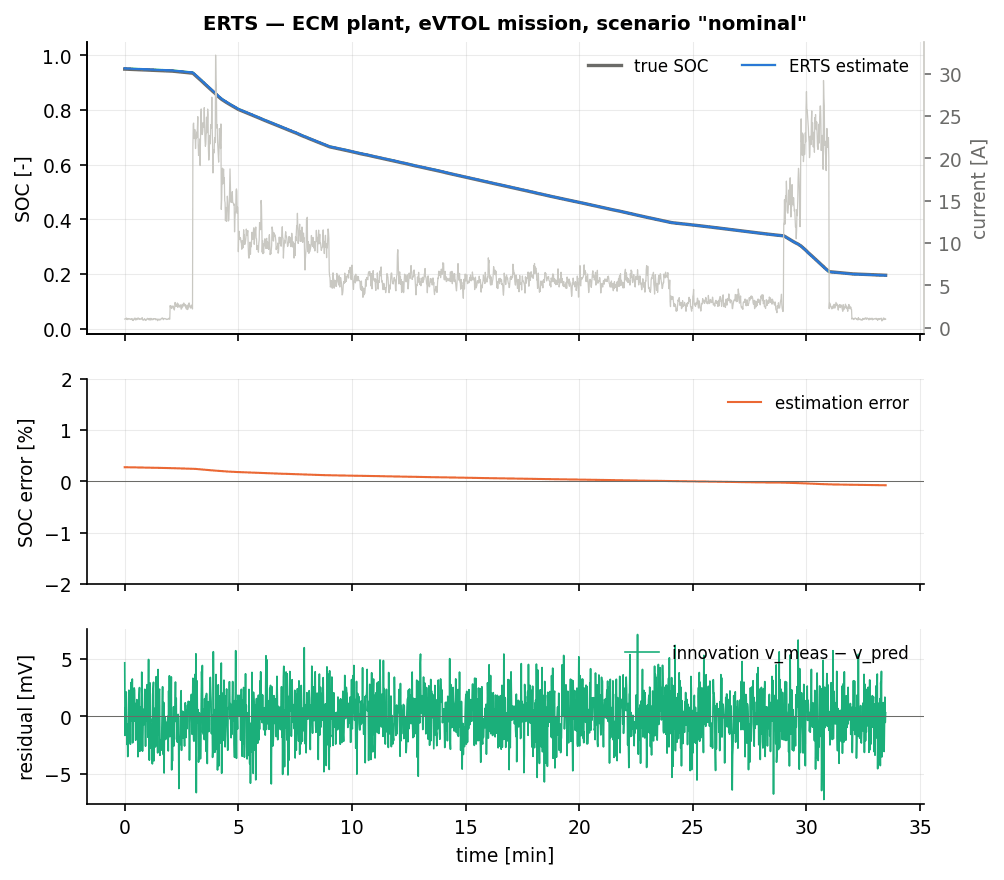
\includegraphics[width=\textwidth]{figures/cell_ERTS_nominal.png}
\caption{ERTS on the nominal eVTOL mission: true and smoothed SOC (top), estimation error with the $\pm 2\sigma$ band (middle), smoothed voltage residual (bottom).}
\end{figure}
\begin{figure}[H]\centering
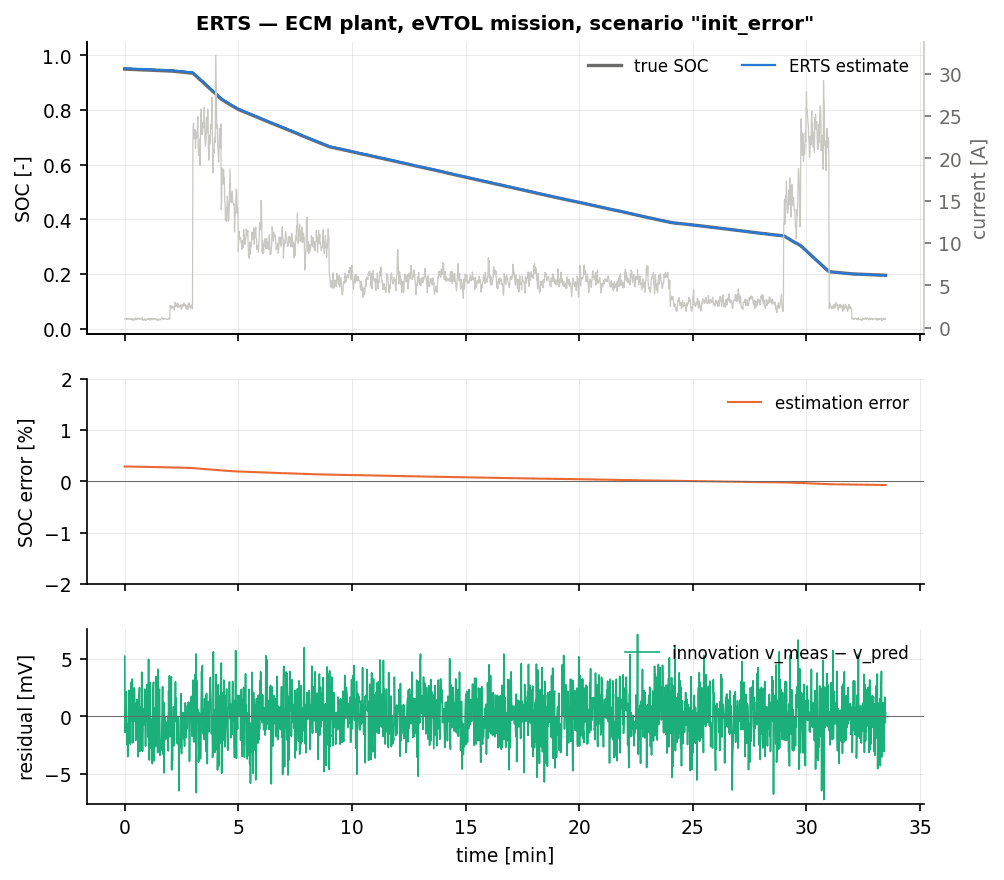
\includegraphics[width=\textwidth]{figures/cell_ERTS_init_error.png}
\caption{ERTS with a \SI{35}{\percent} initial SOC error.}
\end{figure}

\paragraph{Does the smoother smooth?}  The cleanest way to answer is to remove the one error source
that is \emph{not} in the model.  The benchmark's nominal current sensor has a \SI{+0.5}{\percent}
scale-factor error and a \SI{20}{\milli\ampere} offset, neither of which appears in $\mQ$.  Running
the same eVTOL mission with an ideal current sensor gives
\begin{center}
\begin{tabular}{@{}lrrrr@{}}
\toprule
SOC RMSE, ideal current sensor (mean of 3 seeds) & EKF & ERTS & URTS & Batch-NLS\\
\midrule
 & $0.00170$ & $\mathbf{0.00028}$ & $0.00028$ & $0.00040$\\
\bottomrule
\end{tabular}
\end{center}
so the RTS pass reduces the EKF's error by a factor of $6$ when the model is correct --- which is
what the theory promises and confirms the implementation.  All three offline smoothers land within a
factor of $1.4$ of one another here, as they should: for a problem this close to linear, one
linearised backward sweep already recovers almost all of the available information.

\paragraph{The benchmark scenarios.}  All figures are means over three seeds.  On \texttt{nominal} ERTS gives $\text{RMSE}=0.0013$ and
$\text{RMSE}_\text{ss}=0.0004$, converging at $t=0$; the plain EKF measured in the same run gives
$0.0015/0.0005$ and the UKF $0.0020/0.0004$.  On \texttt{init\_error} ERTS gives
$0.0013/0.0004$ with immediate convergence.  Both acceptance criteria are met and nothing diverges
in any seed.

The smoother removes the EKF's start-up transient completely --- the maximum error over the whole
record falls from $0.0132$ to $0.0037$ --- but it replaces it with a small, almost linear bias that
runs from about $+0.0037$ at $t=0$ to $-0.0009$ at the end, which is why the run-average gain over
the filter is much smaller than the correct-model diagnostic above suggests.  This is the central
caveat of this chapter.  That ramp is the signature of the
unmodelled current-sensor scale factor: the smoother believes the Coulomb-counting dynamics almost
exactly (the model's SOC process-noise floor is $\sigma=10^{-5}$ per step) and therefore cannot bend
the trajectory; all it can do is shift it, and the best compromise shift distributes the
\SI{0.5}{\percent}$\times0.75\approx0.0038$ SOC discrepancy over the record.  The filter, which
forgets, ends up with a smaller \emph{average} error even though it is worse at every individual
early sample.  The general statement --- a fixed-interval smoother is only as good as its process
model, and a time-\emph{correlated} input error is the worst case for it --- is the price of using
all the data.

\paragraph{Where smoothing clearly wins.}  \texttt{sensor\_dropout}: $0.0035/0.0030$ against the
EKF's $0.0072/0.0046$, because the \SI{15}{\second} stuck voltage is bracketed by good data on both
sides.  \texttt{current\_bias}: $\text{RMSE}_\text{ss}=0.0041$ against $0.0061$.
\texttt{outliers}: $0.0035/0.0020$ against $0.0052/0.0021$.  \texttt{noise\_step}, \texttt{hot},
\texttt{preisach} and \texttt{param\_mismatch} are all improved.  The smoothed voltage residual is
lower than the filter's in every scenario (\SI{0.73}{\milli\volt} against \SI{0.79}{\milli\volt} on
\texttt{nominal}, \SI{0.73}{\milli\volt} against \SI{2.12}{\milli\volt} on \texttt{init\_error}),
which is the quantity a fault-forensics workflow actually looks at.

\paragraph{Where it loses.}  \texttt{aged\_cell}: $0.0357/0.0159$ against the EKF's
$0.0118/0.0152$.  The mechanism is the same as on \texttt{nominal} but much larger: the model's
capacity is \SI{18}{\percent} too high, so the Coulomb dynamics are systematically wrong, and a
smoother that trusts them spreads the resulting discrepancy over the whole record instead of letting
the OCV feedback absorb it sample by sample.  The \texttt{combined} scenario is worse still
($0.133/0.110$) but for a different reason: there the \emph{forward} EKF fails outright ($0.160$),
and a fixed-interval smoother can only refine what the forward pass produced.  Replacing the forward
EKF by a UKF removes that failure completely --- see Chapter~\ref{ch:urts}, where URTS scores
$0.0099$ on the same scenario --- and that comparison is the strongest practical argument in this
part of the report for choosing the forward filter carefully before reaching for a smoother.

\paragraph{The electrochemical plant.}  On the SPM plant, where the estimator's ECM carries a
structured few-millivolt model error, ERTS gives $\text{RMSE}_\text{ss}=0.0346$ on \texttt{nominal}
against the plain EKF's $0.0373$ --- a marginal gain, and on \texttt{cold} it is actually worse
($0.0914$ against $0.0735$).  The reason is the one already given: a smoother refines a forward
trajectory under the assumption that the process model is right, and on the SPM plant it is not.
The parameter-adaptive filters of Chapters~\ref{ch:jointekf}--\ref{ch:dualukf}, which can move the
model towards the plant, are the better tool there; smoothing and parameter adaptation are
complementary rather than competing.

\paragraph{Re-tuning.}  Because the dominant unmodelled effect is a correlated input error, an
obvious remedy is to inflate the process noise.  Representing a \SI{0.5}{\percent} gain error as an
equivalent white SOC random walk over $N$ steps requires a per-step standard deviation of
$0.005\,\Delta \soc/\sqrt{N}\approx2.7\times10^{-5}$, about $2.7$ times the model's floor, i.e.\ a
variance scale of $\approx4$.  Raising \texttt{opts.q\_scale} to $4$ was measured to improve \texttt{aged\_cell},
\texttt{combined} and \texttt{param\_mismatch} substantially at the cost of a slightly worse steady
state on \texttt{nominal}.  The default is left at $1$ so that ERTS, the EKF and the other smoothers
share identical tuning and the comparison isolates the smoothing, but the knob is exposed and the
derivation above tells the integrator how to size it for a given sensor specification.

Cost: \SI{0.90}{\micro\second}/step, \SI{12.5}{\mega\byte} for the stored trajectory.

\section{Summary}
The extended RTS smoother is the default post-flight tool: two passes over the recorder, fifty lines
of code on top of the EKF, and a factor of $6$ reduction in SOC error when the model is right.
Use it whenever a trajectory --- rather than a live estimate --- is the product: capacity
bookkeeping, fault forensics, ageing-model updates, and as the E-step of an offline parameter
identification.  Do not expect it to repair a forward filter that diverged (it cannot; use URTS),
and be aware that with a rigid process model it will \emph{spread} a time-correlated input error
over the whole record rather than reject it --- which on the aged cell makes its run-average error
larger than the filter's.  If the current sensor's scale factor is not calibrated, inflate
\texttt{q\_scale} or estimate the sensor error explicitly.
